\chapter{Local Optima and Symmetry}\label{ch:symmetry}

\begin{quote}\itshape
Every guarantee so far has been local: EM ascends, gradients are alive,
the filter is exact. None of it says the optimizer arrives anywhere
worth being. This chapter studies the mixture likelihood's geometry ---
the permutation symmetry that makes ``which expert is which'' undefined,
and the symmetric stationary point at which a mixture quietly collapses
into the pooled model it was built to beat. The centerpiece is a
negative result with teeth: on the very task the thesis cares about,
random restarts provably do not help, and the escape requires an
asymmetry you must inject on purpose. The chapter closes with the
package's device for doing so legally --- and with what remains
irreducibly multimodal after all of it, which Part V's multi-seed
protocol treats as variance to be reported, not hidden.
\end{quote}

\section{The landscape has $K!$ of everything}\label{sec:permsym}

\begin{proposition}[Permutation symmetry]\label{prop:perm}
Let $\rho$ be any permutation of $\{1,\dots,K\}$ and let $\rho\theta$
denote a mixture's parameters with components relabeled by $\rho$
(weights or gate outputs, means, scales --- and for the HMM, $\pi_0$ and
both indices of $A$ --- permuted together). Then the likelihood is
invariant: $\ell(\rho\theta) = \ell(\theta)$ for all $\theta$.
Consequently every stationary point, local optimum, and gradient
trajectory has $K!$ images, and ``expert $k$'' is not an identified
statistical quantity.
\end{proposition}

\begin{proof}
The mixture density \eqref{eq:mixdensity} (and the HMM likelihood via
\eqref{eq:preddecomp}) is a sum over components; relabeling permutes the
summands. Gradient flow commutes with the relabeling because the
objective does.
\end{proof}

Two practical corollaries. First, the loss surface is never
single-basined for $K \ge 2$: whatever optimum exists, its mirror images
exist at the same height, with saddles or ridges between them. Second
--- the operational one --- any quantity indexed by raw expert number is
meaningless across independent fits. Chapter~\ref{ch:hmm} met this as
label permutation across walk-forward windows; the repair is worth
restating as a rule: \emph{identification is declared, not discovered.}
The package sorts experts by $\sigma_k$ ascending after every fit
(``expert 0'' \emph{means} the calm expert, by definition), records the
permutation per fold, and aggregates only canonical indices. The
declaration costs one \code{argsort}; its absence costs silent
apples-to-oranges averages in every cross-fit table.

\section{The symmetric stationary point}\label{sec:symtrap}

Permutation twins are benign --- all $K!$ optima are equally good. The
dangerous geometry lives \emph{between} them. Work in the cleanest
setting that exhibits it, which is also the thesis's own planted world
(Proposition~\ref{prop:signflip}): the sign-flip task,
$y = S\beta x + \varepsilon$ with $S = \pm 1$ equiprobable, fit by a
two-expert mixture with linear experts $\mu_i(x) = b_i x$, a gate, and
fixed equal scales.

\begin{proposition}[The pooled point is stationary]\label{prop:pooled}
Consider the population NLL of the two-expert model on the sign-flip
task. At the \emph{pooled point} --- both experts at the pooled
regression solution ($b_1 = b_2 = 0$, since the pooled slope is zero)
and the gate at any state, e.g.\ uniform --- every gradient in the
system vanishes: gate, experts, and (if free) scales.
\end{proposition}

\begin{proof}
With $b_1 = b_2 = 0$ the two experts define \emph{identical} densities
for every sample, so the responsibilities are uninformative:
$r_1 = \pi_1$, $r_2 = \pi_2$ pointwise (Bayes with equal likelihoods
returns the prior). The gate gradient $\pi - r$ (Theorem~\ref{thm:pir})
is identically zero. The expert-$i$ gradient \eqref{eq:mugrad} becomes
$\E\bigl[\pi_i\,(0 - y)x\bigr]/\sigma^2 = -\pi_i \E[yx]/\sigma^2 = 0$,
since the pooled cross-moment $\E[yx] = \beta\,\E[S]\,\E[x^2] = 0$ is
exactly what Proposition~\ref{prop:signflip} established. The scale
gradient \eqref{eq:siggrad} is a responsibility-weighted moment
condition satisfied by the pooled residual variance. Nothing moves.
\end{proof}

The pooled point is not a pathology of bad luck; it is the mixture
disguised as the single model it should dominate --- same predictions,
same NLL, $r \equiv \pi$, gate silent. Two features make it a trap
rather than a curiosity.

\begin{proposition}[The symmetric subspace is invariant]
\label{prop:invariant}
Under gradient flow (or EM, or any update that is a function of the
current parameters through the objective), the subspace
$\mathcal{S} = \{b_1 = b_2\}$ is invariant: a trajectory that starts
with identical experts keeps them identical forever. Within
$\mathcal{S}$, the dynamics reduce to fitting one pooled regressor,
whose optimum on the sign-flip task is the pooled point.
\end{proposition}

\begin{proof}
If $b_1 = b_2$ then the experts' densities coincide sample-wise, so
$r_1 = \pi_1, r_2 = \pi_2$ as above, and the two expert gradients
\eqref{eq:mugrad} are \emph{equal}:
$\partial \NLL/\partial b_1 = \pi_1 g$, $\partial \NLL/\partial b_2 =
\pi_2 g$ with the same $g = -\E[(y - bx)x]/\sigma^2$\dots{} equal up to
the scalar weights, hence --- for the symmetric gate states reachable
from a symmetric start, $\pi_1 = \pi_2 = \tfrac12$ --- identical
updates. Equal parameters plus equal updates stay equal; on
$\mathcal{S}$ the mixture NLL restricted to the common slope $b$ is a
single-Gaussian regression loss, minimized at the pooled slope.
\end{proof}

\begin{whatbreaks}[the collapse you cannot see in the loss]
This failure produces no red flags in the quantities beginners watch.
The loss \emph{decreases} (to the pooled model's respectable-looking
NLL); training is ``stable''; predictions are sensible. What is quietly
false is everything the thesis is about: the experts are clones, the
gate has learned nothing, the mixture's IC on the sign-flip world is
$\approx 0$ where the specialized solution scores $\approx 0.9$. The
tells are in the mixture diagnostics, which is why the package's
dashboard tracks them from step zero: expert output correlation
$\to 1$, both $\hat\sigma_k$ equal (each inflated to the pooled residual
scale --- Chapter~\ref{ch:regimes}'s ``variance of the slope''
reappearing as phantom noise), responsibilities carrying no information
about the true regime (AUC $\approx 0.5$). During the build this
happened exactly as the theory predicts, across \emph{every} seed tried
--- which is the next proposition's point.
\end{whatbreaks}

\section{Why seed diversity fails}\label{sec:seedsfail}

The standard reflex --- restart from a few random seeds, keep the best
--- rests on an assumption: that random initializations land in
different basins, some of them good. Here the assumption breaks
structurally. A fresh initialization puts the two expert networks at
independent random weights, which in \emph{function} space places both
near the same small random function: the experts start
$\varepsilon$-close to the invariant subspace, with $\varepsilon$ the
scale of initialization noise. The dynamics near $\mathcal{S}$ then
factor into a fast component \emph{along} the subspace (both experts
racing to the pooled fit, driven by the full pooled-regression gradient)
and a slow component \emph{transverse} to it, whose growth must be
bootstrapped by the responsibility contrast --- which is itself
proportional to the experts' separation. Small separation $\Rightarrow$
near-uniform $r$ $\Rightarrow$ near-equal expert gradients
$\Rightarrow$ separation grows only at a rate proportional to itself:
exponential escape from an exponentially small seed, which prices each
decade of initial symmetry at a constant \emph{additive} number of
plateau steps. In the computed toy of Figure~\ref{fig:symmetry} the tax
is already $4\times$ the warm start's entire budget at a transverse
asymmetry of $10^{-5}$; in the full model --- deep experts whose
function-space asymmetry is smaller still, stochastic gradients whose
noise the contrast must out-shout, and $\sigma$ calibrated to the pooled
scale precisely when it matters --- the tax compounds past any budget
actually run: in the package's experiments on the symmetric task, no
plain seed ever specialized. Figure~\ref{fig:symmetry} shows both fates
at an equal step budget: the near-symmetric start funnels into the
saddle and sits; the asymmetric start rides straight into a specialized
optimum.

\begin{figure}[t]
  \centering
  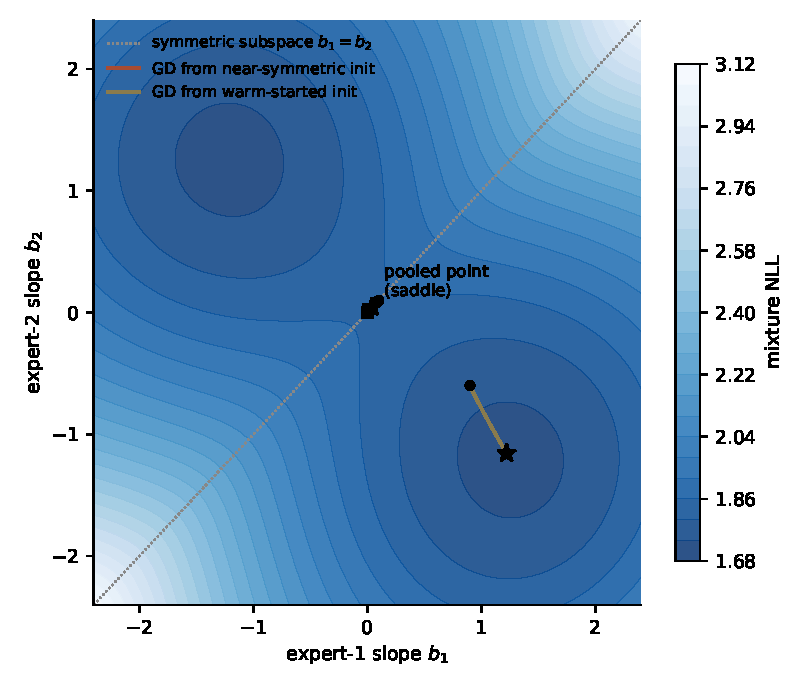
\includegraphics[width=0.8\linewidth]{figures/symmetry_landscape.pdf}
  \caption{\textbf{The symmetric trap, computed.} Mixture NLL over the
  two expert slopes $(b_1, b_2)$ for sign-flip data with a uniform gate
  and the model scale set to $\operatorname{std}(y)$ --- the package's
  \code{sigma\_init} regime, where early-training responsibilities are
  gentle; darker is lower. Twin specialized optima sit near
  $(\pm 1.25, \mp 1.2)$ (pulled inside $\pm\beta$ by the soft
  responsibilities at this $\sigma$); the pooled point $(0,0)$ is a
  saddle on the invariant diagonal (dotted). Both trajectories get the
  same 60-step budget. The warm-started initialization (gold) converges
  in $\sim$50 steps; the near-symmetric initialization (red,
  transverse asymmetry $10^{-5}$) is still pinned at the saddle, and
  needs $\sim$200 steps to escape --- with each further decade of
  initial symmetry costing $\sim$25 more steps, the measured form of
  Exercise~\ref{ex:8-escape}'s exponential-escape law. Seeds move the
  red start by invisible amounts; the warm start moves it across the
  valley.}
  \label{fig:symmetry}
\end{figure}

The statement deserves its honesty clause: this is an argument with a
theorem at its core (the invariance) and dynamics reasoning around it,
not a full proof of basin measure --- and it does not need to be more.
In the package's own experiments on the symmetric task, every plain
seed collapsed and every warm-started run specialized; the design
document records the observation, the test suite pins the warm-started
outcome, and the mechanism above explains rather than merely reports
it.

\section{Breaking symmetry on purpose}\label{sec:warmstart}

If the trap is symmetry, the cure is a deliberate, \emph{legal}
asymmetry. ``Legal'' carries two constraints from earlier chapters: it
must use only training-window information (Chapter~\ref{ch:cross}'s
point-in-time discipline), and it must not supervise the gate (Decision
B --- else the thesis question ``do learned regimes align with real
ones?'' is answered by construction). The package's device threads
both needles:

\begin{center}
\emph{Sort the training window by an observable volatility proxy;
partition into $K$ quantile slices; pre-fit expert $k$ on slice $k$
alone; leave the gate untouched.}
\end{center}

Each ingredient earns its place. The \emph{proxy} (trailing window
volatility on synthetic panels; realized vol or VIX terciles on real
ones) is chosen because Chapter~\ref{ch:regimes}'s entire argument says
volatility is the observable shadow of the latent regime --- the sort
key is correlated with the truth without being the truth. The
\emph{slices} hand each expert a regime-enriched diet, so the pre-fit
experts end up on \emph{opposite sides} of the invariant subspace with
macroscopic separation --- the gold start of
Figure~\ref{fig:symmetry}. The \emph{gate's exclusion} preserves the
experiment: routing must still be discovered by $\pi - r$ from the
likelihood contrast the now-distinct experts create. And the
\emph{mechanics} respect the emission abstraction --- neural experts
pre-train briefly as plain MSE regressors on their slice; classical
Gaussian emissions initialize by their slice's moments in closed form
--- so the device is one polymorphic method, not a special case.

After warm-starting, the previously indistinguishable outcomes separate
cleanly in every diagnostic: on the package's symmetric synthetic task,
responsibility--regime AUC moves from $\approx 0.5$ (every plain seed)
to $\approx 0.99$, the $\hat\sigma_k$ split, and the gate --- never
shown a label --- learns the routing. That last clause is the payoff
worth savoring: symmetry breaking gave the gate something to
distinguish, and Bayes' gradient did the rest.

\begin{engineering}[initialization is epistemology here]
Note what kind of object the warm start is: not a model change (the
architecture is untouched), not a loss change (the objective is the
same NLL), but a \emph{choice of starting point} --- and yet it is the
difference between the thesis model existing and not existing. The
general lesson for non-convex research systems: where the landscape has
structural symmetries, initialization is not a numerical detail but
part of the scientific design, deserving the same documentation,
testing, and pre-registration as the loss. Concretely in the package:
\code{warmstart\_experts} is a first-class, tested trainer method; the
walk-forward harness re-applies it per window from each window's own
training data (no leakage across folds); and the checkpoint/resume
layer stores post-warm-start state so a resumed run never re-runs it.
Its \emph{absence} is equally first-class: the plain-seed collapse is
kept as a documented negative result, because ``we tried the obvious
thing and here is precisely why it fails'' is thesis material, not an
embarrassment.
\end{engineering}

\section{What remains multimodal}\label{sec:remains}

The warm start removes one structural trap. It does not make the
problem convex, and the book's honesty rule requires saying exactly
what is left. Different seeds still reach different interior optima ---
different encoder features, different expert nonlinearities, different
terminal NLLs --- on real data where no planted truth marks one basin
as ``correct.'' The response is not further initialization surgery but
a change of \emph{reporting} category: seed-to-seed dispersion is
treated as genuine model variance, measured by running every
configuration across a seed grid and reported as mean $\pm$ std in
every table (nothing is a result until it has a seed std --- Part V's
first commandment). Local optima thus exit the optimization chapter as
a bug and re-enter the statistics chapters as a variance component ---
which is, in the end, the correct ontology for them.

\begin{codewalk}[nec\_moe/train.py + experts.py --- the warm start]
Trainer side --- build the sort key, slice, delegate:
\begin{lstlisting}
order  = torch.argsort(sort_key)               # vol proxy, train window only
slices = torch.chunk(order, n_experts)         # K quantile slices
self.model.experts.warmstart_slices(x_exp, batch.y, slices, ...)
\end{lstlisting}
Emission side, neural case --- expert $k$ becomes a brief MSE regressor
on its own slice:
\begin{lstlisting}
for _ in range(steps):
    for k, idx in enumerate(slices):
        mu, _ = self(x[idx])
        loss = torch.mean((mu[:, k] - y[idx]) ** 2)   # expert k, slice k
        ...
\end{lstlisting}
The classical emission overrides the same method with two lines of
closed-form moments per slice. What is \emph{not} in either excerpt is
the point: no gate parameter appears anywhere --- Decision B is
enforced by the code's shape, and the symmetry is broken where the
symmetry lives, in the emissions.
\end{codewalk}

\exercisehead

\begin{exercise}\label{ex:8-stationary}
Verify Proposition~\ref{prop:pooled} concretely in torch: build the
two-expert linear mixture on simulated sign-flip data, set
$b_1 = b_2 = 0$ with a uniform gate, and confirm every parameter's
gradient is numerically zero after \code{backward()} on the batch NLL
(up to sampling noise in the finite-sample $\E[yx]$ --- quantify that
noise and pick $n$ to make the point cleanly).
\end{exercise}

\begin{exercise}\label{ex:8-invariant}
Extend Proposition~\ref{prop:invariant} beyond the uniform gate: show
that if $b_1 = b_2$ and the gate is \emph{any} function of $\vh$, the
two experts still receive proportional gradients, and characterize the
full invariant set of the joint (gate, experts) dynamics. What does the
gate converge to within it, and why does that make the collapsed state
even quieter diagnostically?
\end{exercise}

\begin{exercise}\label{ex:8-escape}
Simulate escape times: initialize $(b_1, b_2) = (\varepsilon_0 + \delta,
\varepsilon_0 - \delta)$ for a grid of transverse asymmetries $\delta
\in \{10^{-3}, 10^{-2}, 10^{-1}, 0.5\}$, run gradient descent on the
sign-flip mixture NLL, and record steps-to-specialization (say,
$|b_1 - b_2| > \beta$). Plot log escape time against $\log\delta$ and
reconcile the slope with Section~\ref{sec:seedsfail}'s
``growth rate proportional to separation'' argument.
\end{exercise}

\begin{exercise}\label{ex:8-classical}
Derive the classical emission's warm start in closed form: expert $k$'s
$(\mu_k, \sigma_k)$ from slice $k$'s sample moments. Then show that for
the pure scale-mixture world (means zero, $\sigma_1 \ne \sigma_2$), a
vol-sorted slicing yields $\E[\hat\sigma_1] < \E[\hat\sigma_2]$
strictly --- the warm start lands the classical model on the correct
side of the symmetric subspace with probability approaching one as the
window grows. What property of the sort key is doing all the work?
\end{exercise}

\begin{exercise}\label{ex:8-permcount}
Count the symmetry group precisely for the full thesis model: gate
head, $K$ experts, scales, and (Variation 3) $\pi_0$ and $A$. Beyond
the $K!$ relabelings, does the architecture harbor additional exact
symmetries (hidden-unit permutations inside each expert MLP, sign
flips)? Which of them threaten cross-fit reporting the way label
permutation does, and why does the $\sigma$-sort canonicalization
resolve exactly the dangerous ones?
\end{exercise}

\begin{exercise}\label{ex:8-detector}
Design (then implement against the package) a \emph{collapse detector}:
a boolean diagnostic that fires when a trained mixture is functionally
pooled. Candidate ingredients: expert output correlation, $\sigma$
spread, responsibility entropy, gate-gradient norm. Which single
statistic is hardest to fool, what threshold would you pre-register,
and on which of the package's synthetic worlds (sign-flip, scale-only,
regime-free) must your detector \emph{not} fire despite low expert
disagreement?
\end{exercise}
